% Chapter Template

\chapter{Aplicación de Técnicas y Resultados} % Main chapter title
\label{chap:results} % Change X to a consecutive number; for referencing this chapter elsewhere, use \ref{ChapterX}


%------------------------------------------------   
\section{Introducción}

En este capítulo se realizará la explicación de todas las técnicas aplicadas sobre el dataset. En primer lugar, se detallará cómo se ha realizado la obtención del dataset; en segundo lugar, cómo se ha realizado la aplicación de las técnicas de clustering; en tercer lugar, los resultados obtenidos tras la aplicación del análisis exploratorio de los datos; y en último lugar, cómo se ha realizado la aplicación de las técnicas de forecasting. \\

El código asociado a este capítulo se encuentra en el repositorio público \citep{master}.



%------------------------------------------------   
\section{Obtención del dataset}
\label{sec:data-downloading}

El dataset empleado para este trabajo es un dataset incremental actualizado cada 3 o 4 días, por lo que solo sería necesario descargar el dataset cuando haya sido actualizado. Sin embargo, el volumen de registros añadidos en cada actualización no son significativos para la aplicación de las técnicas de clustering y forecasting, de tal manera que la descarga de los datos se realiza si han pasado, como mínimo, 15 días desde la última descarga del dataset (el número de días es un parámetro configurable). Así, cada vez que se descarga el dataset, el volumen de registros nuevos que sí es significativo para la aplicación de las técnicas de clustering y forecasting. \\

El dataset en formato CSV se almacena dentro de la carpeta \code{src/data/} mientras que la información que viene asociada \citep{dataset} se almacena en la carpeta \\ \code{src/data/info/}. Por último, junto al dataset se almacena el fichero \code{local\_data\_date} con la marca de tiempo en el que se descargó el dataset. Cada vez que se descarga el dataset, el antiguo dataset (y su información asociada) queda almacenado en la carpeta \\ \code{src/data\_backup/}. \\

Todo esto se encuentra implementado en el notebook \code{src/download\_data.ipynb} \citep{master}.


%------------------------------------------------   
\section{Clustering}
\label{sec:results-clustering}

La aplicación de técnicas de clustering permite obtener agrupaciones y relaciones en los datos que a simple vista no se pueden obtener. En esta sección se va a realizar la aplicación del algoritmo de clustering K-Means \citep{scikit-learn}, realizando primero un preprocesamiento de los datos y posteriormente la obtención de algunas métricas sobre los clusters obtenidos. Todo esto se encuentra implementado en el notebook \\ \code{src/clustering-and-data-analysis.ipynb} \citep{master}.


%------------------------------------------------   
\subsection{Preprocesamiento}
\label{sec:clustering-preprocessing}

Antes de poder aplicar el algoritmo de clustering K-Means \citep{scikit-learn}, el dataset debe ser preprocesado. El preprocesamiento de este dataset ha consistido en los siguientes pasos:

\begin{itemize}
 \item \textbf{Rellenar valores nulos}. En el dataset se han encontrado tres tipos de valores nulos: 
 \begin{itemize}
  \item \textbf{Valores de formato fecha}. Han sido rellenados con el valor \code{01/01/1990}.
  \item \textbf{Valores de formato texto}. Han sido rellenados con el valor de la cadena vacía.
  \item \textbf{Valores de formato texto asociados a identificadores}. Han sido rellenados con el valor \code{-1}.
 \end{itemize}
 
 \item \textbf{Eliminar de los registros} con valor distinto de \code{01/01/1990} en los campos \\ \code{DiscontinuedDate} y \code{ChemicalDateRemoved}, pues solo se precisan de aquellos registros de cosméticos que tengan productos químicos y no hayan sido retirados del mercado.

 \item \textbf{Seleccionar las características} expuestas en la Tabla \ref{tab:features-selection}.
 \item \textbf{Agrupar por año y mes} de cada una de las características de formato fecha, sumando los valores del campo \code{ChemicalCount}.
 \item \textbf{Seleccionar características que presenten multicolinealidad} en el dataset aplicando el Factor de Inflación de la Varianza \textit{(Variance Inflation Factor (VIF))} \citep{vif}.
\end{itemize}

Tras aplicar este preprocesamiento, el dataset resultante se compone de 7.487 registros y 7 características, las cuales se muestran en la Tabla \ref{tab:features-preprocessing}, donde \code{\_Year} y \code{\_Month} indican el año y el mes del campo asociado, respectivamente.

\begin{table}[!th]
\begin{tabular}{@{}l@{}}
\toprule
Nombre                                \\ \midrule
\code{InitialDateReported\_Year}      \\
\code{InitialDateReported\_Month}     \\
\code{MostRecentDateReported\_Year}   \\
\code{MostRecentDateReported\_Month}  \\ 
\code{SubCategoryId}                  \\
\code{CasId}                          \\ 
\code{ChemicalCount}                  \\
\bottomrule
\end{tabular}
\centering
\caption{Características del dataset después del preprocesamiento.}
\label{tab:features-preprocessing}
\end{table}





%------------------------------------------------   
\subsection{Aplicación del algoritmo K-Means}

Una vez aplicado el preprocesamiento, tenemos el dataset preparado para poder aplicar el algoritmo de clustering K-Means \citep{scikit-learn}. Sin embargo, este algoritmo necesita que se le proporcione el número de clusters en los que dividir el dataset. Con las características que presenta el dataset no se puede saber el número óptimo de clusters sin aplicar alguna técnica que nos proporcione este número. \\

Para la obtención del número óptimo de clusters, se han utilizado los métodos de la Silueta \textit{(Silhouette Method)} \citep{scikit-learn} y del Codo \textit{(Elbow Method)} \citep{elbow}. En la Figura \ref{fig:silhouette-elbow-methods} se muestran las dos gráficas de la aplicación de los métodos anteriores al dataset. Estas gráficas nos indican que el número óptimo de clusters en los que se divide el dataset es 3. \\

Una vez obtenido el número óptimo de clusters, se puede aplicar el algoritmo K-Means indicándole que el número de clusters es 3. Las Tablas \ref{tab:cluster0}, \ref{tab:cluster1}, \ref{tab:cluster1-1} y \ref{tab:cluster2} muestran la distribución de los productos químicos en los tres clusters tras aplicar el algoritmo. \\

La Figura \ref{fig:clusters-distribution} muestra la distribución de los cluster obtenidos según la relación entre los productos químicos \code{CasId} y los cosméticos \code{SubCategoryId}. Mientras que la Tabla \ref{tab:clusters-distribution} muestra la distribución de los clusters de manera numérica.


\begin{figure}[!th]
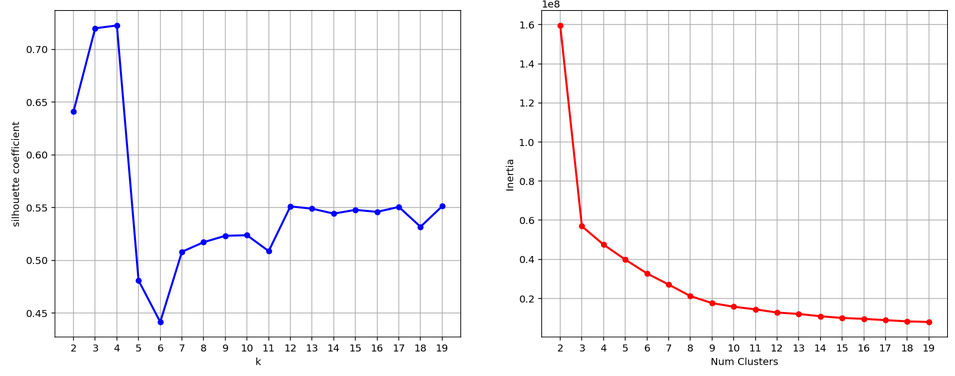
\includegraphics[scale=0.45]{figures/silhouette-elbow-methods}
\centering
\caption{Aplicación de los métodos \textit{Silhouette} (izquierda) y \textit{Elbow} (derecha) para la obtención del número óptimo de clusters.}
\label{fig:silhouette-elbow-methods}
\end{figure}

\begin{figure}[!th]
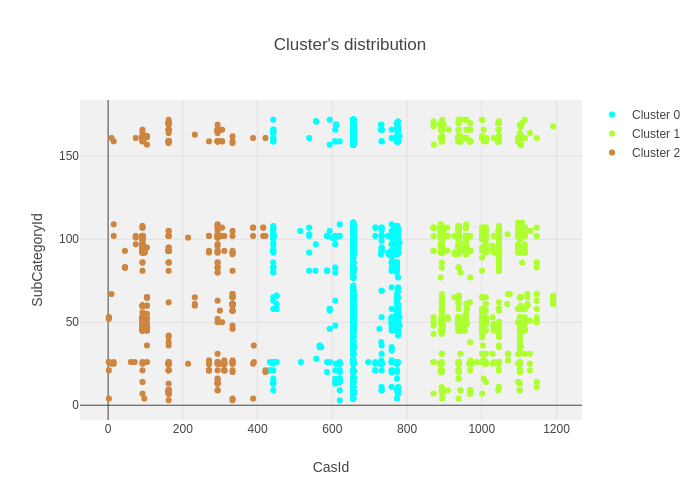
\includegraphics[scale=0.5]{figures/clusters-distribution}
\centering
\caption{Distribución de los clusters según la relación entre los productos químicos \code{CasId} y los cosméticos \code{SubCategoryId}.}
\label{fig:clusters-distribution}
\end{figure}

\begin{table}[!th]
\begin{tabular}{@{}ccc@{}}
\toprule
Cluster 0 & Cluster 1 & Cluster 2 \\ \midrule
5.532 & 1.476 & 479 \\
\bottomrule
\end{tabular}
\centering
\caption{Distribución de los clusters según el número de registros de cada cluster.}
\label{tab:clusters-distribution}
\end{table}



%------------------------------------------------   
\subsection{Métricas del clustering}

Tras aplicar el clustering, se van a calcular ciertas métricas sobre los clusters obtenidos para ofrecer los resultados del clustering de manera más precisa. Las métricas que han sido utilizadas son las siguientes:

\begin{itemize}
 \item \code{Average Within} \citep{metrics}. Mide la distancia media dentro de las observaciones de cada cluster (distancia intra-cluster). Viene definido por la ecuación \ref{eq:average-within}, siendo $K$ el número de clusters, $C_i$ el conjunto de elementos del cluster $i$ y $centroid_i$ el centroide del cluster $i$: 
 \begin{equation}
  SSE = \sum\limits^{K}_{i=1} \sum\limits_{x \in C_i} dist(centroid_i, x)^2
  \label{eq:average-within}
 \end{equation}
 
 \item \code{Dunn Index} \citep{metrics}. Define el ratio entre la distancia mínima inter-cluster y la máxima distancia intra-cluster. Viene definido por la ecuación \ref{eq:dunn-index}, siendo $C$ el conjunto de todos los clusters.
  \begin{equation}
  D(C) = \frac{\min\limits_{C_k, C_l \in C, C_k \neq C_l} (\min\limits_{i,j \in C_k, C_l} dist(i, j))}{\max\limits_{C_m \in C} diam(C_m)}
  \label{eq:dunn-index}
 \end{equation}
\end{itemize}

Así pues, las métricas obtenidas se muestran en la Tabla \ref{tab:metrics}:

\begin{table}[!th]
\begin{tabular}{@{}cc@{}}
\toprule
\code{Average Within} & \code{Dunn Index} \\ \midrule
$0.048633$ & $5.692750 \cdot 10^7$ \\
\bottomrule
\end{tabular}
\centering
\caption{Valores obtenidos para las métricas \code{Average Within} y \code{Dunn Index}.}
\label{tab:metrics}
\end{table}








%------------------------------------------------   
\section{Data Analysis}
\label{sec:results-data-analysis}

El Análisis Exploratorio de Datos \textit{(Exploratory Data Analysis (EDA))} \citep{eda} es muy importante para poder obtener información y conocimiento acerca del dataset. Así pues, en esta sección se van a aplicar distintas técnicas para poder obtener qué productos químicos son los más frecuentes, qué cosméticos son los que presentan mayor número de productos químicos, cómo se distribuyen los datos en función de ciertos campos y cómo se distribuyen por cluster, la cantidad de productos químicos totales. Todo esto se encuentra implementado en el notebook \code{src/clustering-and-data-analysis.ipynb} \citep{master}.



%------------------------------------------------   
\subsection{Obtención de los productos químicos más frecuentes en los cosméticos}
\label{sec:casid-histograms}

La obtención de los productos químicos más frecuentes en los cosméticos se va a realizar realizando histogramas sobre el campo \code{CasId} del dataset. La Figura \ref{fig:histogram-casid-basic} muestra el histograma sobre todo el dataset, donde se puede observar que entre los valores 600 y 700 hay un gran volumen. \\

Concretamente, este volumen se encuentra entre los valores 656 and 658. La Figura \ref{fig:histogram-casid-656-658} muestra el histograma entre dichos valores, donde se puede observar que el volumen se encuentra en el producto químico con \code{CasId} 656, cuyo nombre es: 
\begin{itemize}
 \item \code{656 - Titanium dioxide}.
\end{itemize}

y pertenece al Cluster 0. 

\begin{figure}[!th]
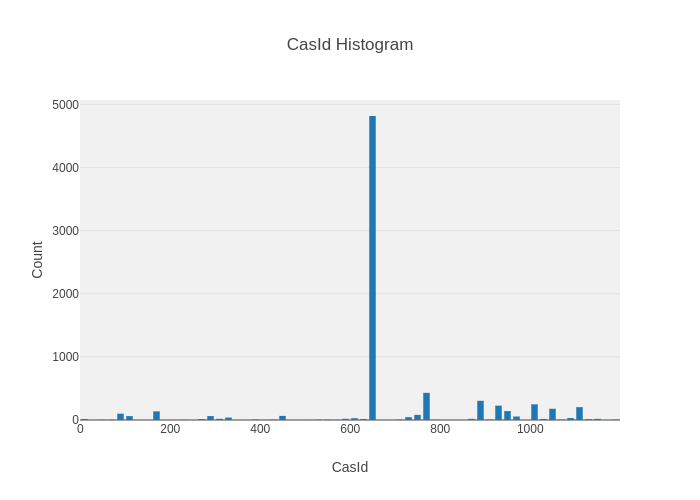
\includegraphics[scale=0.5]{figures/histogram-casid-basic}
\centering
\caption{Histograma sobre el campo \code{CasId}.}
\label{fig:histogram-casid-basic}
\end{figure}

\begin{figure}[!th]
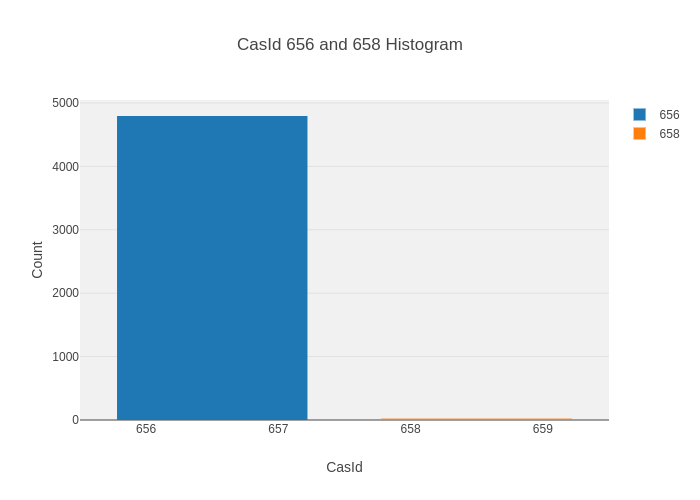
\includegraphics[scale=0.5]{figures/histogram-casid-656-658}
\centering
\caption{Histograma de los valores 656 y 658 del campo \code{CasId}.}
\label{fig:histogram-casid-656-658}
\end{figure}


Sin embargo, como podemos observar en la Figura \ref{fig:histogram-casid-basic}, la diferencia de volumen es muy grande entre el \code{CasId} 656 y el resto. Por lo que se va a realizar los mismos pasos anteriores, pero quitando el \code{CasId} 656 de los datos. \\

La Figura \ref{fig:histogram-casid-without656} muestra el histograma sobre el campo \code{CasId} del dataset sin el \code{CasId} 656 y, además, diferenciando por cluster, donde se puede observar que sigue habiendo un gran volumen entre los valores 700 y 800 y que pertenecen al Cluster 0.


\newpage
\begin{figure}[!th]
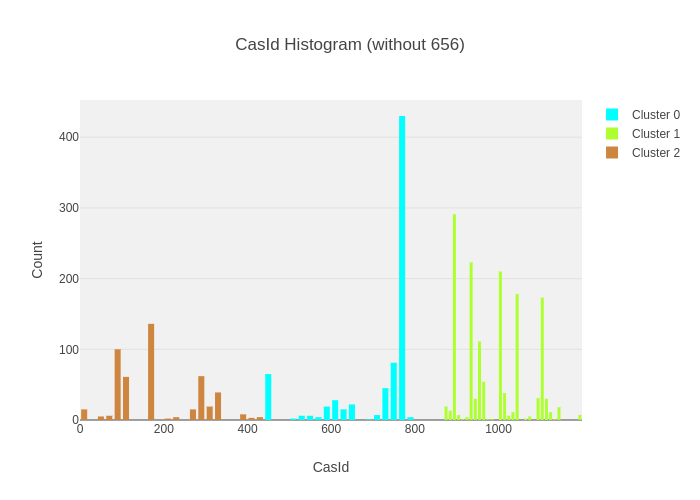
\includegraphics[scale=0.5]{figures/histogram-casid-without656}
\centering
\caption{Histograma sobre el campo \code{CasId} sin el \code{CasId} 656, diferenciando por cluster.}
\label{fig:histogram-casid-without656}
\end{figure}

Concretamente, este volumen se encuentra entre los valores 773 y 776. La Figura \ref{fig:histogram-casid-773-776} muestra el histograma de dichos valores, donde se puede apreciar que el \code{CasId} 773 tiene mayor volumen. El nombre de cada uno de los productos químicos es:

\begin{itemize}
 \item \code{773 - Retinol/retinyl esters, when in daily dosages in excess of 10,000 IU, or 3,000 retinol equivalents}.
 \item \code{776 - Silica, crystalline (airborne particles of respirable size)}.
\end{itemize}


\newpage
\begin{figure}[!th]
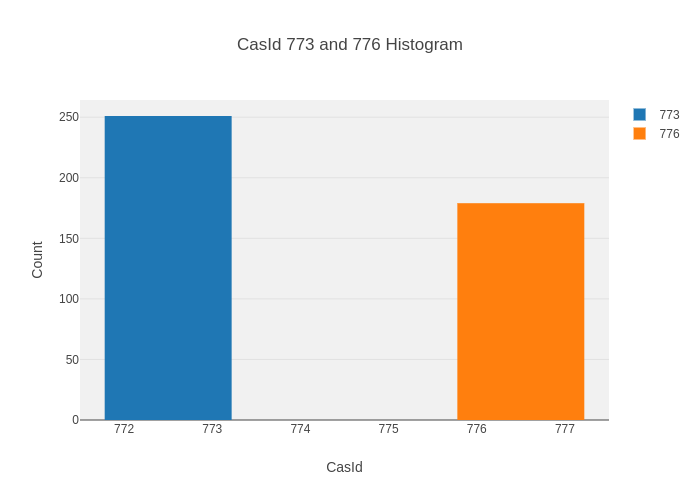
\includegraphics[scale=0.49]{figures/histogram-casid-773-776}
\centering
\caption{Histograma de los valores 773 y 776 del campo \code{CasId}.}
\label{fig:histogram-casid-773-776}
\end{figure}









%------------------------------------------------   
\subsection{Obtención de los cosméticos con mayor número de productos químicos}
\label{sec:subcategoryid-histograms}

Con la misma filosofía que en la sección \ref{sec:casid-histograms}, se van a realizar histogramas sobre el campo \code{SubCategoryId} para obtener los cosméticos que presentan mayor número de productos químicos. La Figura \ref{fig:histogram-subcategoryid-per-cluster} muestra el histograma sobre el campo \code{SubCategoryId} de todo el dataset diferenciando por cluster.

\begin{figure}[!th]
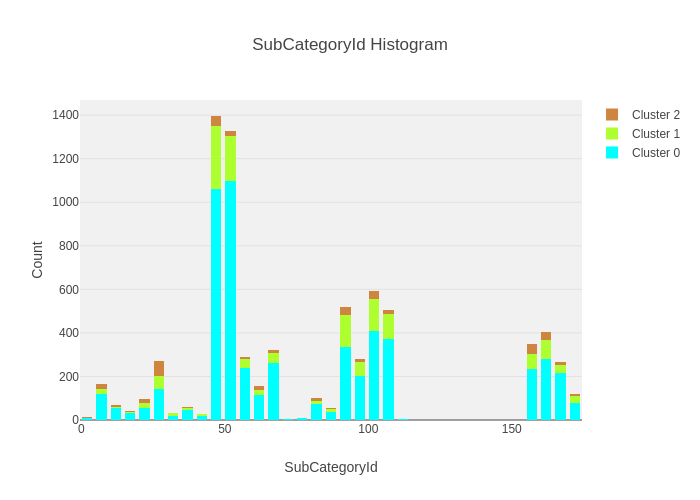
\includegraphics[scale=0.5]{figures/histogram-subcategoryid-per-cluster}
\centering
\caption{Histograma sobre el campo \code{SubCategoryId} diferenciando por cluster.}
\label{fig:histogram-subcategoryid-per-cluster}
\end{figure}


Como se puede observar, hay un gran volumen de registros que pertenecen al Cluster 0, esto es debido al volumen que presenta el \code{CasId} 656 en todo el dataset. Por lo tanto, para poder hacer un estudio más detallado, se va a eliminar el \code{CasId} 656. Así pues, la Figura \ref{fig:histogram-subcategoryid-per-cluster-without656} muestra el mismo histograma que en la Figura \ref{fig:histogram-subcategoryid-per-cluster} pero sin el \code{CasId} 656. 

\begin{figure}[!th]
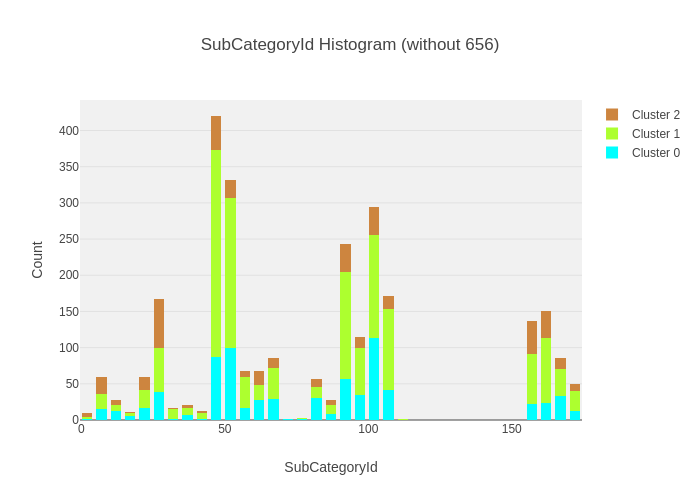
\includegraphics[scale=0.5]{figures/histogram-subcategoryid-per-cluster-without656}
\centering
\caption{Histograma sobre el campo \code{SubCategoryId} diferenciando por cluster, sin el \code{CasId} 656.}
\label{fig:histogram-subcategoryid-per-cluster-without656}
\end{figure}

Al igual que ocurrió con el campo \code{CasId}, se puede observar que entre los valores 40 y 50 del campo \code{SubCategoryId} se encuentra un volumen superior al resto. Concretamente, se encuentra entre los valores 45, 46, 48 y 49. La Figura \ref{fig:histogram-subcategoryid-45-49} muestra el histograma de dichos valores, donde se puede apreciar que el valor \code{SubCategoryId} 48 es el que tiene un volumen mayor. Además, también se puede observar que la gran mayoría de los registros pertenecen al Cluster 1. \\

El nombre de cada uno de los cosméticos es:

\begin{itemize}
 \item \code{45 - Blushes}.
 \item \code{46 - Eyeliner/Eyebrow Pencils}.
 \item \code{48 - Eye Shadow}.
 \item \code{49 - Face Powders}.
\end{itemize}


\newpage
\begin{figure}[!th]
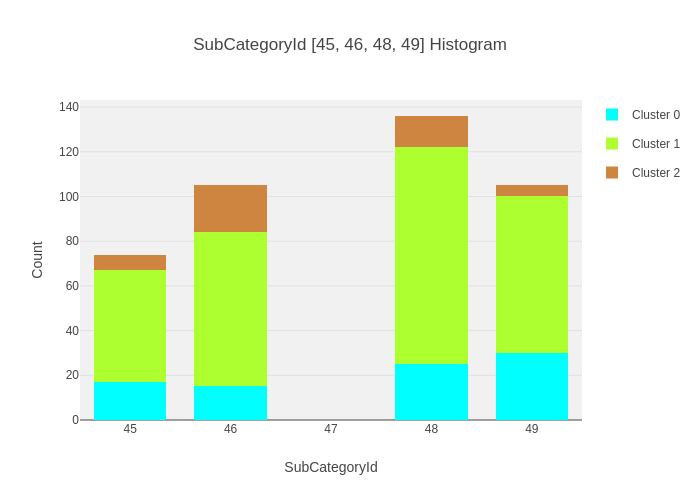
\includegraphics[scale=0.5]{figures/histogram-subcategoryid-45-49}
\centering
\caption{Histograma de los valores 45, 46, 48 y 49 del campo \code{SubCategoryId} diferenciando por cluster, sin el \code{CasId} 656.}
\label{fig:histogram-subcategoryid-45-49}
\end{figure}



\newpage
%------------------------------------------------   
\subsection{Distribución del dataset}
\label{sec:dataset-distribution}

En la Figura \ref{fig:splom-data-aggregated} se muestra la distribución del dataset en función de los campos \code{CasId}, \code{InitialDateReported\_Year}, \code{MostRecentDateReported\_Year} y \code{SubCategoryId}, diferenciando por cluster, en el que se puede observar que en los primeros años (2009 y 2010) fue cuando se reportaron la gran mayoría de los productos químicos y que en los años siguientes han ido reportándose de una manera muy equilibrada.

\begin{figure}[!th]
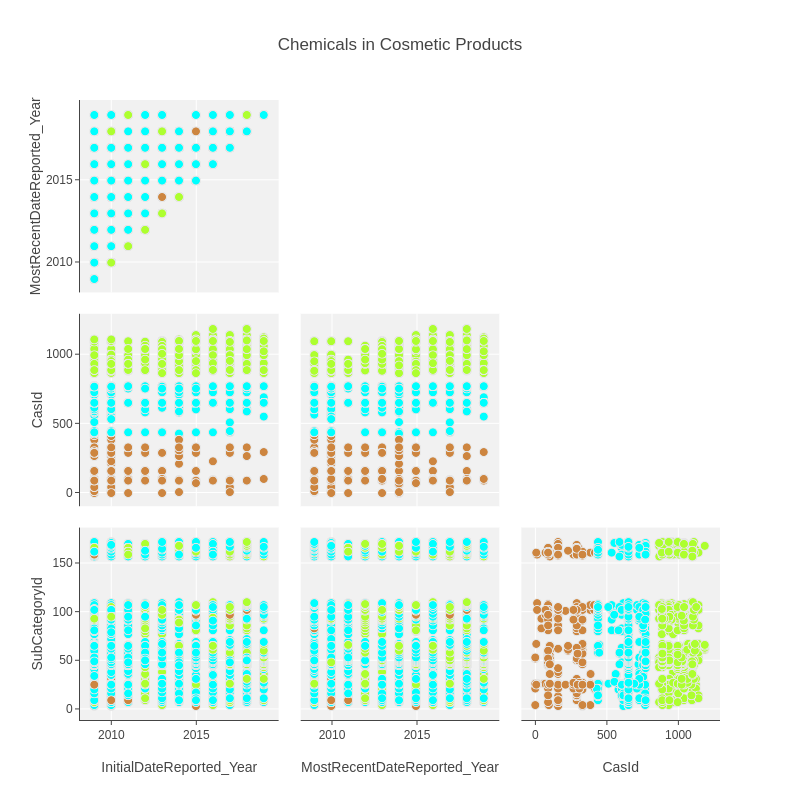
\includegraphics[scale=0.5]{figures/splom-data-aggregated}
\centering
\caption{Distribución del dataset en función de los campos \code{InitialDateReported\_Year}, \code{MostRecentDateReported\_Year}, \code{SubCategoryId} y \code{CasId}.}
\label{fig:splom-data-aggregated}
\end{figure}




\newpage
%------------------------------------------------   
\subsection{Distribución de la cantidad de productos químicos por cluster}
\label{sec:chemicals-per-cluster}

Hasta ahora se han estudiado la frecuencia en la que aparecen los productos químicos y los cosméticos en el dataset. En este punto, se va a estudiar la distribución de la cantidad de productos químicos en cada uno de los clusters, esto es: la suma del campo \code{ChemicalCount} distribuido en cada uno de los clusters. La Figura \ref{fig:pie-sum-chemicalcount} muestra esta distribución.


\begin{figure}[!th]
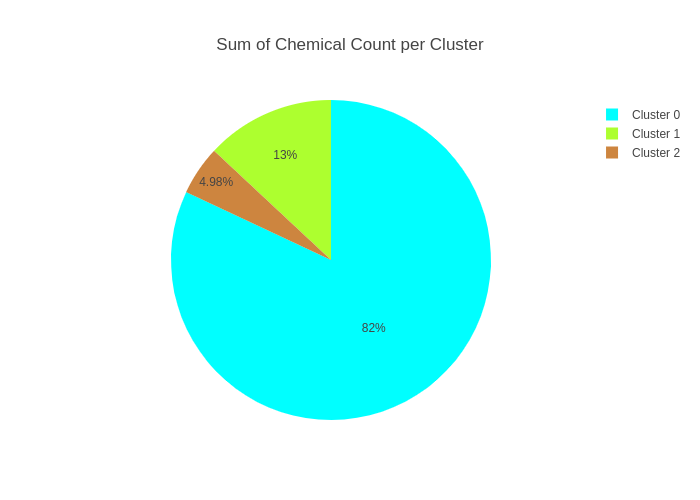
\includegraphics[scale=0.46]{figures/pie-sum-chemicalcount}
\centering
\caption{Distribución de la suma del campo \code{ChemicalCount} por cada cluster.}
\label{fig:pie-sum-chemicalcount}
\end{figure}

Al igual que pasaba en la sección \ref{sec:subcategoryid-histograms}, el alto porcentaje del Cluster 0 se debe al \code{CasId} 656. Por lo que, la Figura \ref{fig:pie-sum-chemicalcount-without656} muestra la misma distribución eliminando el \code{CasId} 656 del dataset. Donde se puede observar que más del 50\% de los productos químicos se encuentran en el Cluster 1.

\begin{figure}[!th]
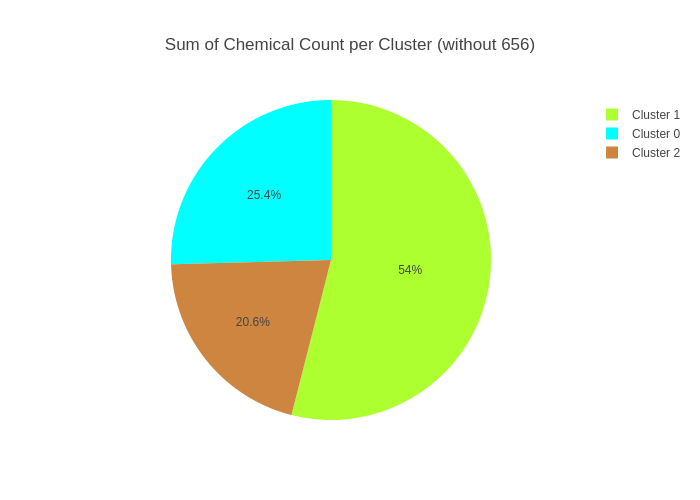
\includegraphics[scale=0.46]{figures/pie-sum-chemicalcount-without656}
\centering
\caption{Distribución de la suma del campo \code{ChemicalCount} por cada cluster, sin el \code{CasId} 656.}
\label{fig:pie-sum-chemicalcount-without656}
\end{figure}

\newpage

%------------------------------------------------   
\section{Forecasting}





%------------------------------------------------   
\subsection{Preprocesamiento}

Antes de poder aplicar el algoritmo de forecasting ARIMA \citep{arima}, el dataset debe ser preprocesado, al igual que se realizó con el clustering en la sección \ref{sec:clustering-preprocessing}. Sin embargo, no se ha realizado el mismo preprocesamiento. A continuación se detallan los pasos realizados en este preprocesamiento:

\begin{itemize}
 \item \textbf{Rellenar valores nulos}. En el dataset se han encontrado tres tipos de valores nulos: 
 \begin{itemize}
  \item \textbf{Valores de formato fecha}. Han sido rellenados con el valor \code{01/01/1990}.
  \item \textbf{Valores de formato texto}. Han sido rellenados con el valor de la cadena vacía.
  \item \textbf{Valores de formato texto asociados a identificadores}. Han sido rellenados con el valor \code{-1}.
 \end{itemize}
 
 \item \textbf{Eliminar de los registros} con valor distinto de \code{01/01/1990} en los campos \\ \code{DiscontinuedDate} y \code{ChemicalDateRemoved}, pues solo se precisan de aquellos registros de cosméticos que tengan productos químicos y no hayan sido retirados del mercado.

 \item \textbf{Agrupar por el campo} \code{InitialDateReported} sumando los valores del campo \\ \code{ChemicalCount}. Ya que el objetivo de la aplicación de forecasting es poder obtener una predicción de la cantidad de productos químicos que serán reportados en el futuro.
\end{itemize}

Tras aplicar este preprocesamiento nos queda un dataset con 1.863 registros y 2 características: \code{InitialDateReported} y \code{ChemicalCount}.




%------------------------------------------------   
\subsection{Obtención de los datasets de entrenamiento y validación}


Para poder realizar el forecasting, se necesita tener datos de entrenamiento y datos de validación (en adelante, \code{dataset} y \code{validation}, respectivamente). La obtención de estos datasets está ligada a que el dataset \citep{dataset} es incremental y se tienen almacenados dos versiones del dataset, como se ha comentado en la sección \ref{sec:data-downloading}. \\ 

Así, se disponen de las siguientes versiones del dataset:

\begin{itemize}
 \item Carpeta \code{src/data/} \citep{master}, donde se almacena la versión más reciente del dataset.
 \item Carpeta \code{src/data\_backup/} \citep{master}, donde se almacena la versión anterior del dataset.
\end{itemize}












\newpage
%------------------------------------------------   
\subsection{Aplicación del algoritmo ARIMA}

















